\documentclass[a4paper,12pt]{article}
\usepackage[T1]{fontenc}
\usepackage[utf8]{inputenc}
\usepackage[ngerman]{babel}
\usepackage[pdftex]{hyperref}
\usepackage{floatflt}
\usepackage{graphicx}
\usepackage{tabularx}
\usepackage{xcolor}
\usepackage{framed}
\usepackage{changes}
\usepackage{tikz}
\usepackage{capt-of}
\usepackage{diagbox}
\usetikzlibrary{arrows.meta}
\usepackage[thmmarks, thref]{ntheorem}
\usepackage{amsmath, amssymb}
\usepackage{eurosym}
%\usepackage[amsmath, thmmarks, thref]{ntheorem}
\usepackage{verbatim}
\usepackage{fancyhdr}
\usepackage[hang]{footmisc}
\renewcommand{\subsectionmark}[\thepage]{\markright{{#1}}}
\textheight220mm
\headheight 28pt
\textwidth160mm
\oddsidemargin0mm
\evensidemargin0mm
\topmargin0mm
\pagestyle{headings}
\fancyhead[R]{\sectionmark}
\newcommand{\F}{\mathbb F}
\newcommand{\f}{\mathbb f}
\newcommand{\K}{\mathbb K}
\newcommand{\R}{\mathcal R}
\newcommand{\N}{\mathbb N}
\newcommand{\Z}{\mathbb Z}
\newcommand{\Q}{\mathbb Q}
\newcommand{\A}{\mathcal A}
\newcommand{\C}{\mathcal C}
\newcommand{\D}{\mathcal D}
\newcommand{\X}{\mathcal X}
\newcommand{\Y}{\mathcal Y}
\newcommand{\xL}{\mathcal L}
\newcommand{\xP}{\mathcal P}
\newcounter{Hilfssatz}
\newcounter{Definition}
\newcounter{Beispiel}
\newcounter{Satz}
\newcounter{Algorithmus}



\setlength{\parindent}{0pt}
\makeatletter
  \@addtoreset{Definition}{subsection}
\makeatother
\newenvironment{Definition}{
\bigskip
        
        \setlength{\parindent}{0pt}
        \addtocounter{Definition}{1}
        \textbf{\textsf{Definition \thesubsection.\theDefinition}:}\\}{
        \nopagebreak
        \vspace{-1.0ex}
        \bigskip
        
}
\makeatletter
  \@addtoreset{Hilfssatz}{subsection}
\makeatother
\newenvironment{Hilfssatz}{
\medskip
        
        \setlength{\parindent}{0pt}
        \addtocounter{Hilfssatz}{1}
        \textbf{\textsf{Hilfssatz \thesubsection.\theHilfssatz}:}\\}{
        \nopagebreak
        \vspace{-1.0ex}
        \bigskip\\
        
}

\makeatletter
  \@addtoreset{Satz}{subsection}
\makeatother
\newenvironment{Satz}{
\medskip
        
        \setlength{\parindent}{0pt}
        \addtocounter{Satz}{1}
        \textbf{\textsf{Satz \thesubsection.\theSatz}:}\\}{
        \nopagebreak
        \vspace{-1.0ex}
        \bigskip\\
        
}

\makeatletter
  \@addtoreset{Beispiel}{subsection}
\makeatother
\newenvironment{Beispiel}{
\medskip
        
        \setlength{\parindent}{0pt}
        \addtocounter{Beispiel}{1}
        \textbf{\textsf{Beispiel \thesubsection.\theBeispiel}:}\\}{
        \nopagebreak
        \vspace{-1.0ex}
        \bigskip
        
}

\setlength{\parindent}{0pt}
\newenvironment{proof}{
\bigskip
        
        \setlength{\parindent}{0pt}
        \textbf{Beweis:}\\}{
        \nopagebreak
        \vspace{-1.0ex}
        \begin{flushright}
             $\square$
        \end{flushright}
        \bigskip
        
}

\makeatletter
  \@addtoreset{Algorithmus}{subsection}
\makeatother
\newenvironment{Algorithmus}{
\medskip
        
        \setlength{\parindent}{0pt}
        \addtocounter{Algorithmus}{1}
        \textbf{\textsf{Algorithmus \thesubsection.\theAlgorithmus}:}}{
        \nopagebreak
        \vspace{-1.0ex}
        \bigskip
        
}

\usepackage{lastpage}% F\"ur die Verweise innerhalb des  Symbolverzeichnisses

\usepackage{nomencl} % Symbolverzeichnis
\let\symb\nomenclature %% Es genuegt \symb statt \nomenclature zu  schreiben
\setlength{\nomlabelwidth}{.25\hsize}
\renewcommand{\nomlabel}[1]{#1 \dotfill}
\setlength{\nomitemsep}{-\parsep}\renewcommand{\nomname}
{Symbolverzeichnis}

\setlength{\nomitemsep}{-\parsep}
\usepackage{array} %notwendig um neue Spaltentypen zu definieren
\newcolumntype{B}[1]{>{\centering\arraybackslash}m{#1}}
\makenomenclature



%Bsp für reelle Zahlen
\begin{document}
\begin{titlepage}
\thispagestyle{empty} \enlargethispage{1.4in}

\begin{center}

\rule[1ex]{157.5mm}{0.5mm}

\LARGE\bf Hochschule für angewandte Wissenschaften Coburg\\

\vfill

\rm Institut für Informatik


\begin{figure}
	    \centering
				     
\includegraphics[width=0.5\textwidth]{Logo.png}
\end{figure}

\vfill

\Huge \bf Projektbericht Datamining

\vfill

\normalsize Michael Krasser

\vfill

Betreuer:  Dr.~Detlef~Bittner

Abgabe des Berichts: 22 Januar 2019

\vfill

Coburg, \today

\rule[-1ex]{157.5mm}{0.5mm}

\vfill

\end{center}

\end{titlepage}

\newpage
\tableofcontents
\pagebreak
\section{Geschäftsverständnis}
\subsection{Beschreibung der Situation}
Das zu untersuchende System beschreibt einen Onlineshop dessen Produktpalette aus Medien wie z.B. CDs, Bücher, Hörbücher, ebooks und ebook-Readern besteht. Um gegenüber großen Online-Anbietern wettbewerbsfähig zu sein muß der Onlineshop regelmäßig Maßnahmen zur Aquise und Kundenbindung ergreifen. Eine Möglichkeit zur Kundenbindung besteht in einer Gutscheinausstellung. 

\subsubsection{Problembeschreibung}
Viele Kunden tätigen meist nur eine Bestellung im Onlineshop. Es kann keine Vorhersage darüber getroffen werden ob ein Kunde eine weitere Bestellung tätigen oder sein Interesse an den Produkten des Onlineshops erlischt. Das Ziel dieser Arbeit besteht in der Bestimmung der Loyalität des einzelnen Kunden anhand von Merkmalen die sich aus den beigelegten Datensätzen erschließen lassen. Ist die Wahrscheinlichkeit sehr gering, dass ein Kunde einen weiteren Einkauf tätigt, erscheint es sinnvoll diesen mittels eines Gutscheins an den Onlineshop zu erinnern. Ist dagegen die Wahrscheinlicht eines erneuten Einkaufs eher hoch, so verursacht die Zusendung eines Gutscheins nur unnötige Kosten.  
\par
Um dieses Problem zu lösen, soll mittels des CRISP-DM Modells \cite{crisp}
und des Datamining-Tools SPSS von IBM eine Bewertung durchgeführt werden, welche die
Loyalität des Kunden bestimmen soll. Hierfür wurden zwei *.txt-Dateien über Kundendaten geliefert.
Als Lösung wird eine Abbildung der Kundennummer auf das zu erwartende Kaufverhalten gefordert. 

Der abschließenden Vergleich kann über den Realdatzensatz Datei dmc2010$\_$real.txt geführt werden, welcher das reale Kaufverhalten dokumentiert.
\subsection{Situationsbewertung}

\subsubsection{Beschreibung der gelieferten Daten}
Bei den zur Verfügung gestellten Daten  handelt es sich um Auszüge aus den Bestelldaten einer Kundendatenbank.
Es gibt Spalten für das Datum einer Lieferung, Accounterstellung und der
ersten Bestellung, Domain und Kundennummer des Kunden und eine Reihe von Flags, die das Kaufverhalten des Kunden beschreiben:
Es wird registriert ob gebrauchte oder importierte Artikel gekauft wurden, wie die Ware zum Kunden gelangt ist, wie der Kunde bezahlt hat, ob die Lieferung zurückgeschickt oder gecancelt wurde und wie viele Artikel der Kunde auf einmal gekauft hat.

\subsubsection{Risikofaktoren}

Das Risiko des Onlineshops liegt in der Versendung zu vieler Gutscheine. Diese Gutscheine können dann auch Kunden erreichen, die auch ohne diese wieder eine Bestellung getätigt hätten. In diesem Fall verliert der Shop pro Bestellung 5 \euro. Je nachdem, wie viele der Gutscheine unnötig ausgegeben werden, kann
sich diese Vorgehensweise als unrentabel erweisen. (Einfluß des falsch positiven und des falsch negativen Fehlers bleiben unberücksichtigt.)

\subsubsection{Erfolgskriterien}
Es konnten drei zentrale Erfolgskriterien für das Projekt identifiziert werden:
\begin{itemize}
	\item Entscheidung ob ein Kunde einen Gutschein erhält
	\item Maximierung des Gewinns im Datensatz dmc2010 class.txt
	\item Ab einem Gewinn von 9.310,50\euro\; im Testdatensatz und 8547,50\euro\; im class-Datensatz\footnote{Dieser Werte wird ebenfalls mit Gl.$(\ref{gl1})$  aus dmc2010$\_$real.txt ermittelt.} liegt ein erfolgreiches Datamining vor
\end{itemize}

\textbf{Bemerkung}:
\par
Zur Berechnung des Gewinnes (bzw. des Verlustes) wurde folgende Entscheidungsmatrix vorgeschrieben:

\begin{table}[h]
\begin{center}
\begin{tabular}{c | c | c }
 &$\overline{\text{Wiederkäufer}}$\footnotemark & Wiederkäufer
\\
\hline
Gutschein & 1.5 & -5
\\
$\overline{\text{Gutschein}}$ & 0 & 0
\end{tabular}
\caption{Zugelieferte Entscheidungsmatrix}
\end{center}
\end{table}
\footnotetext{Das überstrichene Symbol ist hier und im folgenden als mathematisches Komplement zu verstehen.}
Ein an eine Person, die von alleine nicht wieder bestellt, ausgegebener Gutschein bedeutet für den Onlineshop einen Gewinn von 1,50 \euro\;. Jeder Kunde der fälschlicherweise
einen Gutschein bekommt, ergibt einen Verlust in  Höhe des Wertes des Gutscheins, also 5 \euro.

Als Referenzwert\label{Referenzwerte} für die Modellbildung wird folgende Situation
zugrunde gelegt: Jeder Kunde erhält einen Gutschein. Unter der Annahme, dass jeder dieser Kunden auch wieder eine Bestellung tätigt, erhält man im Testdatensatz (26377 Kunden tätigten keine weitere Bestellung innerhalb von 90 Tagen, 6051 aber schon) einen Verlust von
\begin{align}
(26377 *1.50 - 6051*5)\;\text{\euro} = 9310,50\;\text{\euro}\label{gl1}
\end{align}
Diese Werte müssen in der Modellbildung übertroffen werden.

\subsection{Projektplanung}
Für die Projektdurchführung wurde zu Projektbeginn der Aufwand in
Wochen für die jeweiligen Projektschritte des CRISP-DM Modells geschätzt:
\begin{itemize}
	\item Geschäftsverständnis: ca zwei Wochen
	\item Datenverständnis: ca zwei Wochen
	\item Datenvorbereitung: ca zwei Wochen
	\item Modellbildung: ca eineinhalb Wochen
	\item Evaluierung und Bereitstellung: ca eine halbe Woche
\end{itemize}

\section{Datenverständnis}
\subsection{Datensammlung}
Einige Feler des Datensatzes sind weniger erfolgsversprechend als andere. Da bereits eine
Beschreibung der einzelnen Felder zugeliefert wurde, kann an dieser Stelle eine Vorsortierung
der Spalten erfolgen. Um versehentliche Korrelationen mit unwichtigen Daten im Ergebnis der
Untersuchung zu vermeiden, sollten diese vor der Betrachtung aussortiert werden.



\subsubsection{Vernachlässigbare Felder}
Unwichtige Felder lassen sich anhand verschiedener Merkmale identifizieren. Bei einer
auffallend schlechten Datenqualität sollte das Feld aussortiert\footnote{Die Entfernung erfolgte mittels eines Typ-Knotens im SPSS Modeler.} werden(fehlende Einträge, Ausreisser).
Außerdem existieren Felder, anhand deren Beschreibung bereits erkannt werden
kann, dass diese keinen Einfluß auf das Ergebnis haben können. Als solche Felder wurden die im folgenden beschriebenen identifiziert:
\par
\vspace{1cm}
\begin{minipage}[h]{.5\textwidth}
\begin{itemize}
	\item "`salutation"'
	\item "`domain"'
	\item "`model"'
	\item "`invoicepostcode"'
	\item "`delivpostcode"'
\end{itemize}
\end{minipage}
\hfill
\begin{minipage}[h]{.5\textwidth}
\begin{itemize}
  \item "`advertisingdatacode"'
	\item "`points"'
	\item "`shippingcosts"'
	\item "`weight"'
	\item "`used"'
	\end{itemize}
\end{minipage}
\par
\vspace{1cm}
Die Anrede ("`salutation"') wurde zu Beginn als relevant eingestuft, in einem späteren Analyseschritt aber entfernt:
Email-Domain oder Anrede  eines Kunden haben sicher wenig bis gar keinen Einfluß auf das Kaufverhalten des Kunden. Die Bedeutung des Feldes "`model"' konnte nicht schlüssig geklärt werden, daher wurde es auf Grund des vernachlässigbaren Prädikatoreinflusses entfernt.
Die Rechnungsadresse ("`invoicepostcode"') und die Lieferadresse ("`delivpostcode"') wurden auch verworfen da hier keine Rückschlüsse auf das Kaufverhalten des Kunden erkennbar sind. Außerdem erwies sich die Datenqualität des Feldes "`invoicepostcode"' als schlecht wegen vieler NULL-Werte.
Der Werbecode ( "`advertisingdatacode"') wurde auf Grund schlechter Datenqualität entfernt. Punkte eingelöst ("`points"') schien zunächst relevant, da es Aufschluss über die Empfänglichkeit des Kunden für Werbeaktionen gibt, erwies sich aber als nicht hilfreich und wurde in einem späteren Schritt auf Grund der der zu schlechtene Datenqualität entfernt. Spezifische Artikelinformation wie Versandkosten ("`shippingcosts"') Gewicht ("`weight"') und Second Hand ("`used"') wurden auch entfernt, da sich hieraus keinerlei Information ableiten ließ.

Zusätzlich wurden die Produktkategorien w0 - w10 gleich zu Beginn als uniteressant für die Modellbildung eingestuft.


\subsubsection{Erfolgsversprechende Felder}
Bewertet wurde die Datenqualität, die Datenplausibilität und der
Vorteil, den die Daten für die Auswertung ergeben könnten. Das Feld "`datecreated"' kann in Verbindung
mit dem Feld "`date"' dazu genutzt werden, um die Zeit zwischen der Accounterstellung
und der ersten Bestellung zu berechnen. Daher werden beide Attribute beibehalten. Auch aus
den Feldern "`cancel"', "`deliverydatepromised"', "`deliverydatereal"'
etc. können zusammengesetzte Felder ermittelt werden.
Zusätzlich sollten die Spalten "`gift"', "`voucher"' und "`newsletter"' für die Auswertung verwendet werden, da sie Aufschluss über das Kaufverhalten des Kunden geben: Durch das Feld
"`newsletter"' kann beispielsweise erkannt werden, ob der Kunde generell über Interesse an den Produkten
des Shops verfügt. 

\subsection{Datenbeschreibung}

\subsubsection{Datenmenge}
Im Trainingsdatensatz und dem Vorhersagedatensatz befinden sich 32.428 bzw. 32.427 Datensätze.
Datenmengen dieser Größe sind für eine vollständige Analyse im Sinne von Big Data nicht
ausreichend, was sich auch in der späteren Modellierung der Daten zeigte.

\subsubsection{Untersuchung der Daten}

Jede Zeile der Dateien liefert Informationen über eine Bestellung. Jede Bestellung lässt sich eindeutig einem Kunden mittels des
Feldes "`customernumber"' zuordnen. Anhand der angegebenen Werte der Bestellung lässt sich
feststellen, ob die versprochene Lieferzeit eingehalten wurde, welche Artikel bestellt wurden
und wie sich diese zusammensetzen. Weitere Daten sind indirekt enthalten und lassen sich aus vorhandenen Daten ermitteln.

\subsubsection{Konsistenz}
Felder mit schlechter Datenqualität (fehlende Werte, NULL-Werte, viele Ausreisser,\ldots) sollten unter Verwendung eines Filters entfernt werden.
Hierzu gehören die Felder "` points "`und "`advertisingdatacode"' (viele fehlende Werte), "`invoicepostcode"' und "`deliverydatereal"' (NULL-Werte).
Jedoch mussten diese beiden Felder zunächst für die Datenvorbereitung zur Erzeugung neuer Attribute beibehalten werden.

\section{Vorbereitung der Daten}
\subsection{Bereinigung der Daten}
Die Bereinigung der Daten erfolgte in zwei Schritten: 
\par
Zunächst wurden alle NULL-Werte aussortiert und danach Extremwerte (Ausreißer).
Die Wertemenge einiger Felder enthielt viele NULL-Werte welche bei der späteren Modellierung hinderlich sein könnten.
Entsprechend wurden diese Werte (z.B bei "`deliverydatereal"' und "`deliverydatepromised"') mit einem Auswahl-Knoten des SPSS Modelers entfernt, 
was eine deutliche Reduzierung der Datenmenge nach sich zog: Etwa 7000 Datensätze  wurden entfernt.
Unrealistische Werte wurden ebenfalls mit dem Auswahl-Knoten entfernt.

\subsection{Erstellung neuer Felder}
\begin{figure}[h]
	    \centering
				     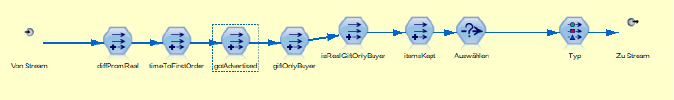
\includegraphics[width=\textwidth]{Datenvorbereitung.png}
						\captionof{figure}{Erstellte Felder}
\end{figure}


Durch studieren der Situation konnten neue Felder aus bestehenden Feldern gebildet\footnote{Der Ableiten-Knotens des SPSS Modelers bietet die Möglichkeit neue Felder mittels minimaler Programmierung zu erstellen.} werden:  
\begin{framed}
\begin{verbatim}
diffPromReal = deliverydatepromised - deliverydatereal
\end{verbatim}
\end{framed}
Differenz aus versprochenem und tatsächlichem Lieferdatum: Liegt das tatsächliche Lieferdatum nach dem versprochenen ist die Wahrscheinlichkeit recht groß den Kunden zu verlieren. 
\begin{framed}
\begin{verbatim}
timeToFirstOrder = datecreated - date
\end{verbatim}
\end{framed}
Zeitdauer zwischen Registrierung des Kunden und seiner ersten Bestellung.
\begin{framed}
\begin{verbatim}
gotAdvertised = newsletter OR voucher
\end{verbatim}
\end{framed}
Aufschluss ob Kunde an Werbemaßnahmen teilnimmt.
\begin{framed}
\begin{verbatim}
giftOnlyBuyer = gift AND (numberitems == 1) 
\end{verbatim}
\end{framed}
Aufschluss ob Kunde ein Geschenk bestellt hat.
\begin{framed}
\begin{verbatim}
isRealGiftOnlyBuyer = (giftOnlyBuyer == 1) AND (date == datecreated)
\end{verbatim}
\end{framed}
Aufschluss ob Kunde sich nur für die Bestellung eines Geschenks registriert hat.
\begin{framed}
\begin{verbatim}
itemsKept = numberitems - remi - cancel 
\end{verbatim}
\end{framed}
Aufschluss  über die Anzahl der Artikel die der Kunde bestellt und auch behalten hat.


\newpage
\subsection{Bewertung der Felder}

Nachdem neue Felder erstellt wurden, muss der Einfluss dieser auf die Modellierung bewertet werden.
Hierfür wurde nach der Datenvorbereitung  ein Knoten zur Merkmalauswahl angefügt.

Dabei ergab sich, dass 10 der 19 Felder als bedeutsam (100 \%) eingestuft wurden, ein weiteres Feld besaß eine Korrelation von über 90 \%,
die restlichen wurden als unbedeutsam (Korrelation von unter 90\%) eingestuft.
Korrelationswerte sollten lediglich als Richtlinie betrachtet werden, da die Gewichtung
vieler Attribute bei 100\% lag.  Unter den 10 bedeutsamen Feldern befanden sich auch einige der
generierten:

\vspace{0.2cm}
\par
	\begin{minipage}[h]{.5\textwidth}
	\begin{center}
	"`itemsKept"'
	\end{center}
	\end{minipage}
	\hfill
	\begin{minipage}[h]{.5\textwidth}
	\begin{center}
	"`gotAdvertised"'
	\end{center}
	\end{minipage}
	\vspace{0.2cm}
\par
Damit stehen für die Modellierung zehn Felder zu Verfügung:
\begin{center}
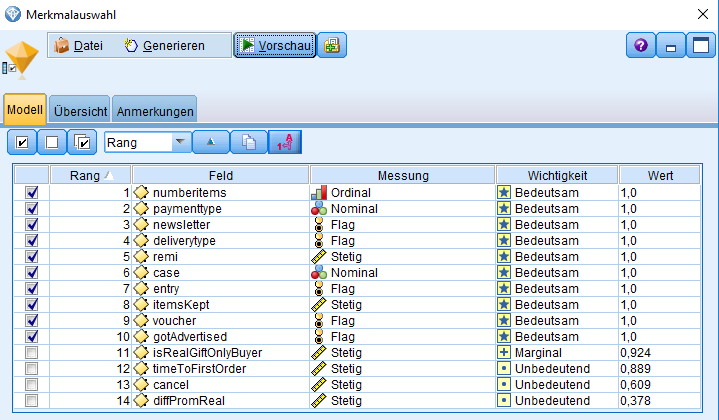
\includegraphics[width=\textwidth]{Screens/Merkmalauswahl}
\captionof{figure}{Merkmalauswahl}
\end{center}

\section{Modellierung}
Als Grundlage für die Modellierung werden die unter ~\ref{Referenzwerte} ermittelten Referenzwerte verwendet. Ziel der Modellierung ist eine Maximierung des Gewinns, also ein Modell zu entwickeln, dessen Gewinn die berechneten Gewinne übertrifft.  
\subsection{Wahl der Modellierungsknoten}
Die Erklärungen zu den einzelnen Knoten sind \cite{nodes} entnommen und können dort nachgelesen werden. 
Hinsichtlich der Struktur der Aufgabe kann man sich auf Baummodelle bei der Wahl der Knoten im SPSS Modeler beschränken. Hierfür wurden folgende Modellierungsknoten in Betracht gezogen:
\begin{itemize}
\item CHAID
\item C5.0
	\item Random-Trees
	\item XGBoost-Baum
\end{itemize} 

Anfänglich  wurden alle von SPSS Modeler zu Verfügung gestellten Modellierungsknoten betrachtet, aber nicht alle lieferten brauchbare
Ergebnisse: Die Support Vector Machine (SVM) lieferte viele NULL-Werte.
\par
Hinsichtlich der Validierung wurde zusätzlich überprüft, ob sich die getroffene Merkmalauswahl positiv auf den erzielten Gewinn auswirken konnte. Dabei konnte erkannt werden, welche Felder welchen Einfluß auf die Modellierung besitzen.
\subsection{Test-Design}
Ziel der Testausführung ist eine automatisierte Auswertung der verwendeten Modellierungsknoten aus den Datensätzen:
Das jeweilige Modell-Nugget erstellt das Feld \$R-Target90\$ aus dem class Datensatz welches anschließend mit dem realen Feld target90 verglichen werden soll.
Zu diesem Zweck wird die Entscheidungstabelle modifiziert:
\begin{center}
\begin{tabular}{c | c | c}
target90 & \$R-target90\$ & Betrag
\\
\hline
0 & 0 & 1.5
\\
\hline
0 & 1 & 0
\\
\hline
1 & 0 & -5
\\
\hline
1 & 1  & 0
\end{tabular}
\end{center}
Der Wert 0 im Feld \$R-target90\$ bedeutet die Vorhersage, dass ein Kunde keine erneute Bestellung tätigt.
\begin{center}
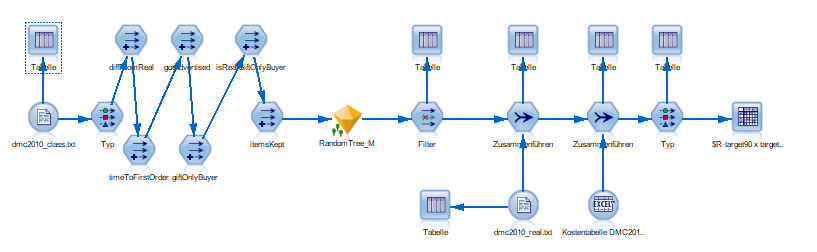
\includegraphics[width=\textwidth]{Screens/test_bewertung}
\captionof{figure}{Modellierung des Testdesigns}
\end{center}

\subsubsection{CHAID}
{\bf Erklärung}:
\par
\vspace{0.2cm}
Der CHAID-Knoten generiert Entscheidungsbäume unter der Verwendung der $\chi^2$  - Verteilung.
Im Gegensatz zum C\&R-Baum  und QUEST können mit diesem Modell auch nicht binäre Bäume generiert werden, d.h. Bäume mit mehr als zwei
Verzweigungen. Berücksichtigt wurde das Verhalten des Gewinnes unter Merkmalauswahl und Boosting auf dem class Datensatz. 

\begin{center}
\begin{tabular}{ c | c | c }
 & Boosting & $\overline{\text{Boosting}}$
\\
\hline
Merkwahlauswahl  &  8,548.50\;\euro & 8,575.00\;\euro
\\
$\overline{\text{Merkwahlauswahl}}$ & 8,697.00\;\euro  &  8,548.50\;\euro
\\
\end{tabular}
\end{center}

\begin{center}
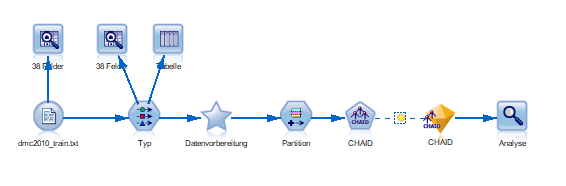
\includegraphics[width=\textwidth]{Screens/chaid}
\captionof{figure}{CHAID-Modellierung - ohne Merkmalauswahl}
\end{center}

\begin{center}
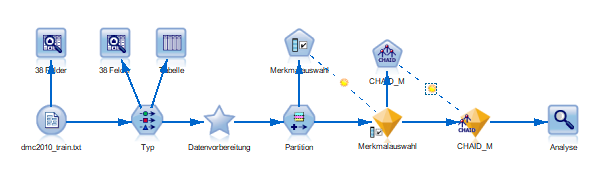
\includegraphics[width=\textwidth]{Screens/chaid_m}
\captionof{figure}{CHAID-Modellierung - mit Merkmalauswahl}
\end{center}

{\bf Auswirkung der Merkmalauswahl}:
\par
\vspace{0.2cm}
Die Verwendung der Merkmalauswahl produziert ein schlechteres Ergebnis als ohne diese, d.h. die Merkmalauswahl für dieses Modell wurde unpassend gewählt.
\par
\vspace{0.2cm}

{\bf Auswirkung der Fehlklassifizierung:}
\par
\vspace{0.2cm}
Bei Baummodellen kann eine Gewichtung der Fehlklassifikationen vorgenommen werden. Diese
Gewichtung dient der Anpassung, indem eine Fehlklassifizierung höhere
Kosten bedeutet. Ohne vorgeschaltete Merkmalauswahl und ohne Boosting bei einer Fehlklassifizierung mit dem Faktor 3.0 berechnet der CHAID-Algorithmus einen Gewinn von 8,548.50\;\euro\;
was zu keiner Verbesserung führt.

\subsubsection{C5.0}
{\bf Erklärung}:
\par
\vspace{0.2cm}
Der C5.0-Algorithmus, erstellt einen Entscheidungsbaum oder ein Regelset.
 Ein C5.0-Modell teilt die Stichprobe auf der Basis des Felds auf, das den maximalen
Informationsgewinn liefert. Jede durch die erste Aufteilung definierte Teilstichprobe wird anschließend
wieder aufgeteilt, üblicherweise auf der Grundlage eines anderen Felds. Der Prozess wird so lange fortgesetzt,
bis die Unterstichproben nicht weiter aufgeteilt werden können. Zum Schluss werden die Aufteilungen
der untersten Ebene noch einmal untersucht, wobei solche entfernt oder reduziert werden, die nicht
wesentlich zum Wert des Modells beitragen.
\par
\vspace{1cm}
Mit dem C5.0-Algorithmus konnten auf dem class Datensatz 9,055.00\;\euro\; Gewinn errechnet werden, also eine deutliche Verbesserung gegenüber der Vorhersage des CHAID-Knotens.

\begin{center}
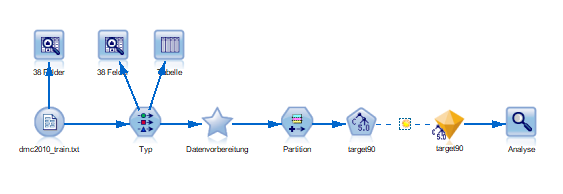
\includegraphics[width=\textwidth]{Screens/c50}
\captionof{figure}{C5.0 - ohne Merkmalauswahl}
\end{center}

\begin{center}
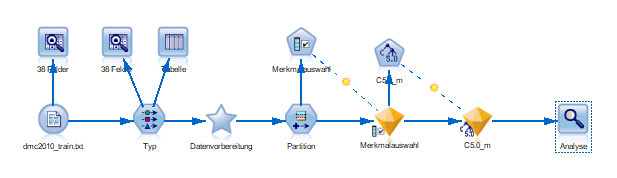
\includegraphics[width=\textwidth]{Screens/c50_m}
\captionof{figure}{C5.0 - mit Merkmalauswahl}
\end{center}

{\bf Auswirkung der Merkmalauswahl}:
\par
Im Gegensatz zum CHAID-Algorithmus, verbessert eine vorgeschaltete Merkmalauswahl hier den vorhergesagten Gewinn: Ohne vorgeschaltete Merkmalauswahl erziehlt der Algorithmus 8,548.50\;\euro\; Gewinn, mit dieser sogar 8,732.00\;\euro\; auf dem class Datensatz.
\par
\vspace{0.2cm}

{\bf Auswirkung der Fehlklassifizierung:}
\par
 Bei einer Fehlklassifizierung mit dem Faktor 3.0 berechnet der C5.0-Algorithmus einen Gewinn von 9,028.50\;\euro,\; mit vorgeschalteter Merkmalauswahl erhält man sogar einen Gewinn von 9,055.00\;\euro\; auf dem class Datensatz.

\subsubsection{Random-Trees}
{\bf Erklärung}:
\par
\vspace{0.2cm}
Dieser Knoten erwies sich als bester Modellierungsknoten.
Der Algorithmus entwickelt ein Modell, welches sich aus verschiedenen Entscheidungsbäumen zusammensetzt.
Random Trees entspricht in der grundlegenden Vorghensweise der des C\&R-Baums, erweitert
diesen jedoch um zwei Punkte: Zum einen wird in diesem Modell Bagging verwendet, um
ein Overfitting des Datensatzes zu vermeiden. Zum anderen wird für jede Aufteilung des Baums
lediglich eine Stichprobe der Input-Werte zur Errechnung der Unreinheit benutzt.
Mittels dieses Modells konnten auf dem class Datensatz maximal 10,143.50 \euro\;  Gewinn vorhergesagt werden:

\begin{center}
	\begin{tabular}{l | c | c | c}
	
	Fehlklassifizierungskosten & -- &  1.0 &  3.0
	\\
	\hline
	Merkmalauswahl  & 10,113.50\;\euro  & 10,143.50\;\euro & 10,143.50\;\euro
	\\
	$\overline{Merkmalauswahl}$  & 10,109.00\;\euro &  10,109.00\;\euro & 10,109.00\;\euro
	
	\end{tabular}
\end{center}

\begin{center}
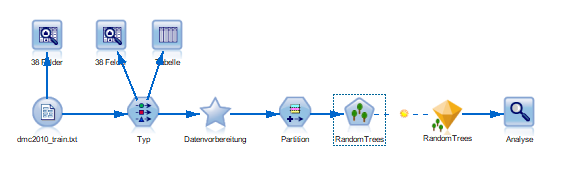
\includegraphics[width=\textwidth]{Screens/random_trees}
\captionof{figure}{Random-Trees Modellierung}
\end{center}

{\bf Auswirkung der Merkmalauswahl und der Fehlklassifizierungskosten}:
\par
Bei Verwendung der Merkmalauswahl liefert der Random Trees-Algorithmus leicht bessere Ergebnisse.
Daran lässt sich erkennen, dass die Merkmalauswahl für dieses Modell sinvoll gewählt wurde.
Eine zusätzliche Verwendung der Fehlklassifizierungskosten verbesserte das Ergebnis ebenfalls, eine Erhöhung der Gewichtung mit dem Faktor 3.0 lieferte allerdings keine weitere Verbesserung.

\begin{center}
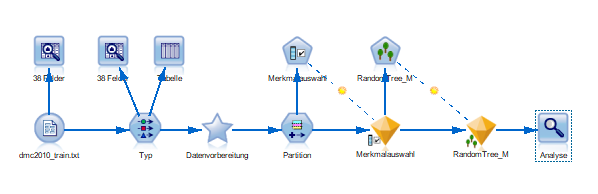
\includegraphics[width=\textwidth]{Screens/random_trees_m}
\captionof{figure}{Random-Trees Modellierung mit Merkmalauswahl}
\end{center}

\subsubsection{XGBoost-Baum}
{\bf Erklärung}:
\par
\vspace{0.2cm}
Dieser Modellierungsknoten ist die erweiterte Implementierung eines Gradienten-Boosting-Algorithmus mit einem
Baummodell als Basismodell. Boosting-Algorithmen lernen iterativ schwache Klassifikationsmerkmale
und fügen Sie einem endgültigen starken Klassifikationsmerkmal hinzu.



\section{Evaluierung und Bereitstellung}

\newpage
\section{Tabellenverzeichnis}
\listoftables 


\newpage
\section{Abbildungsverzeichnis}
\listoffigures
\addcontentsline{toc}{section}{Abbildungsverzeichnis}
\newpage

\newpage
\section{Literaturverzeichnis}
\thispagestyle{plain}
\begin{thebibliography}{DiplRS}
\bibitem[1]{crisp} {\it CRISP-DM: Ein Standard-Prozess-Modell für Data Mining} \url{ https://statistik-dresden.de/archives/1128}.
\bibitem[2]{nodes} {\it IBM SPSS Modeler 18.1 Modellierungsknoten} 
\url{ftp://public.dhe.ibm.com/software/analytics/spss/documentation/modeler/18.1/de/ModelerModelingNodes.pdf}
\end{thebibliography}

\newpage
\begin{titlepage}
\section*{Erklärung:}
\noindent {\large Die vorliegende Projektarbeit wurde am Institut für Informatik  der Hochschule Coburg nach einem Thema von Herrn Dr.~Detlef~Bittner erstellt.
\newline Hiermit versichere ich, dass ich diese Arbeit selbstständig angefertigt und dazu nur die angegebenen Quellen verwendet habe.

\vspace{1.5cm}

\noindent Coburg, den \today

\vspace{0.5cm}

\raggedleft Michael Krasser\quad\quad \par}

\vfill
\end{titlepage}
\end{document}
